\documentclass{beamer}
\usepackage[utf8]{inputenc}
\usepackage{tikz}
\usepackage[most]{tcolorbox}
\usetikzlibrary{positioning}
\usepackage{cleveref}
\numberwithin{equation}{theorem}

\title{Fast and accurate numerical solvers for oscillatory ODEs}
\date{\today}
\author{\textbf{Fruzsina Agocs}\inst{1}, with Alex Barnett\inst{1}}
\institute{\inst{1} Center for Computational Mathematics, Flatiron Institute, Simons Foundation
}

\usetheme{CCM}

\begin{document}

\begin{frame}
	\titlepage
\end{frame}

%\begin{frame}
%	\begin{itemize}
%		\item Hi
%	\end{itemize}
%	\begin{theorem}[Theorem 1]
%		Proof of Theorem 1
%	\end{theorem}
%\end{frame}

\begin{noframe}
    The problem and existing methods to solve it  
    \smallskip
    {\footnotesize
    \begin{itemize}
        \item{Interested in solving the general linear 2nd order ODE
        \begin{align}\label{ode}
            &u''(t) + \gamma(t)u'(t) + \omega^2(t)u(t) = 0, \quad t \in (t_i, t_f) \nonumber \\
            &\text{with} \quad u(t_i) = u_i, \quad u'(t_f) = u_f.
        \end{align}
       } 
       \item{When $\omega \gg 1$, $u(x)$ is oscillatory, conventional ODE solvers need discretization with $\mathcal{O}(\omega)$ steps $\rightarrow$ slow,}
       \item{Some efficient solvers for high-frequency case: cite Bremer, cite Arnold++, cite Petzold, cite oscode, maybe QML}
       \item{All except oscode and Arnold++ (which references oscode) only applicable in the high $\omega$ regime}
       \item{All except oscode and Petzold only applicable in the $\gamma(t) = 0$ case}
       \item{Bremer is the only arbitrarily high-order method (oscode is $\mathcal{O}(h)$, Arnold $\mathcal{O}(h^2)$) }
       \item{\textbf{This work:} applicable in both oscillatory and slowly-changing regimes, $\gamma \neq 0$ allowed, arbitrarily high order}
    \end{itemize}
    }
\end{noframe}

\begin{noframe}
    Method overview \medskip
    {\footnotesize
    \begin{itemize} 
    \item{Two separate time-stepping methods to deal with $\omega \gg 1$ and $\omega = \mathcal{O}(1)$ with adaptive switching between them and adaptive stepsize}
    \item{$\omega = \mathcal{O}(1)$: Spectral method based on Chebyshev nodes }
    \item{$\omega \gg 1$: Asymptotic expansion for a nonoscillatory phase function:}
    \item{Rewrite \cref{ode} ($\gamma(t) = 0$) using $u = e^z$, and $z'(t) = x(t)$ being the \emph{phase function}:
    \begin{equation}
        x'(t) + x^2(t) + \omega^2(t) = 0, \quad \text{(Riccati)}
    \end{equation}
    }
    \item{Solutions generally oscillatory, but Bremer+Rokhlin have shown that there exist nonoscillatory phase functions for analytic $\omega(t)$}
    \item{They define the phase function $\alpha(t)$ as  $$u(t) = \cos(\alpha(t))/\sqrt{\alpha(t)},\quad \sin(\alpha(t))/\sqrt{\alpha(t)},$$ and construct a nonoscillatory $\alpha$ by solving the third order ODE it satisfies with appropriate i.c.}
    \item{\textbf{This work:} construct approximate, nonoscillatory $x^{(k)}(t)$, $k=0, 1, \ldots$ by functional iteration, without explicit reference to i.c.  }
    \end{itemize}
    }
\end{noframe}

\begin{noframe}
    Method overview II \medskip
    {\footnotesize
    \begin{itemize}
    \item{If $\omega \gg 1$, approximate nonoscillatory solutions: $x(t) \approx \pm i\omega $ } 
    \item{Therefore let zeroth order solutions be $x_0 = \pm i\omega$}
    \item{Define residual of \cref{ode} as
    \begin{equation}
    R[x(t)] \equiv R[x] = x' + x^2 + \omega^2,
    \end{equation}
    then 
    \begin{equation}
    R[x_k + \delta] = R[x_k] + \delta' + 2x_k \delta + \mathcal{O}(\delta^2)
    \end{equation}
    }
    \item{Set to 0. After linearisation, $\delta$ solves an ODE which again is generally oscillatory}
    \item{But if $\delta$ nonoscillatory, $\delta'$ is $\mathcal{O}(\omega)$ smaller than other terms $\rightarrow$ neglect,}
    \item{Get Newton-like, functional defect correction scheme:
    \begin{equation}
    x_{k+1} = x_k - \frac{R[x_k]}{2x_k}
    \end{equation}
    }
    \item{Sanity check: if $x = \mathcal{O}(\omega)$, $\omega' = \mathcal{O}(\omega)$, then
    \begin{align}
    x_0 &= i\omega, \quad R[x_0] = i\omega' = \mathcal{O}(\omega),\\ 
    x_1 &= i\omega - \frac{\omega'}{2\omega}, \quad R[x_1] = -\frac{\omega''}{2\omega} + \frac{3(\omega')^2}{4\omega^2} = \mathcal{O}(1).
    \end{align}
    }
    \end{itemize}
    }
\end{noframe}

\begin{noframe}
	Examples I: Airy equation, $y'' + yt = 0$
	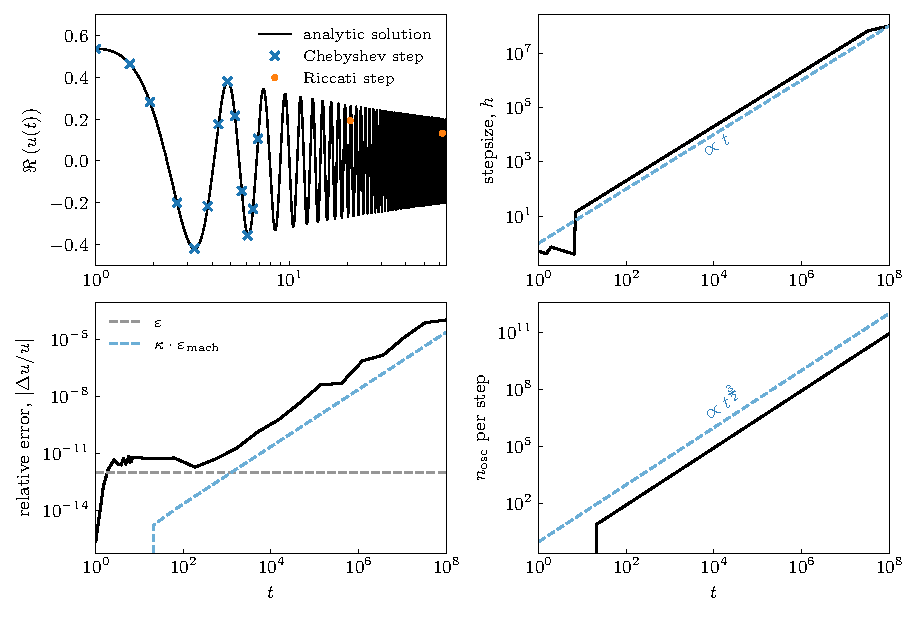
\includegraphics[]{airy-numsol.pdf}
\end{noframe}

\begin{noframe}%[b]
	%Bottom justified frame - Beamer understands where the blue bar is.
	Examples II: Burst equation, $y'' + \frac{n^2 - 1}{(1 + t^2)^2}y = 0$
	\includegraphics[]{burst-numsol.pdf}
\end{noframe}

\begin{noframe}
    Legendre polynomial figure here
\end{noframe}

\begin{noframe}
    Examples IV: Ideas  \\
    \medskip
    {\footnotesize
    Cosmology: Mukhanov--Sasaki equation and primordial power spectra (PPS)
    \begin{itemize}
    \item{Describes time-evolution of spacetime curvature perturbations during inflation ($\approx 10^{-34}$ s after Big Bang)}
    \item{Has highly oscillatory region followed by a slowly-varying phase}
    \item{Quantity of interest is PPS, for which the ODE needs to be solved $\mathcal{O}(10^3)$ times, each for a different Fourier mode}
    \item{For Bayesian inference, a PPS needs to be generated for each parameter vector $\rightarrow$ overall $\mathcal{O}(10^9)$ ODE solves}
    \end{itemize}
    Quantum mechanics: time-independent, one-dimensional Schr\"{o}dinger equation
    \begin{itemize}
    \item{Could solve the ODE from two points lying outside the potential well, going inwards, with an initial energy guess $E$,}
    \item{Then check for continuity at a midway point $\rightarrow$ turn into optimisation / root finding problem for finding energy eigenvalues}
    \end{itemize}
    }
\end{noframe}

\begin{noframe}
    \begin{minipage}{0.5\textwidth}
    Details: the algorithm \\ 
    \vphantom{.} \\
    {\scriptsize
    In stepping from $t_i$ to $t_{i+1} = t_i + h$:
    \begin{enumerate}
        \item Get initial stepsize estimate
        \item Refine stepsize estimate
        \begin{itemize}
            \item \scriptsize $h_{\text{slo}}$: Halve $h$ until maximum $1/\omega(t)$ over $(t_i, t_i +h)$ is no larger than $\sigma/\omega(t_i)$ (with $\sigma = 1.2$)
            \item  \scriptsize$h_{\text{osc}}$: Iterate over number of Chebyshev nodes until $\omega(t)$ can be interpolated to within $\epsilon_h$ over $(t_i, t_i+h)$ ($\epsilon_h$ typically $10^{-12}$)
        \end{itemize}
        \item Decide whether to attempt Riccati step
        \begin{enumerate}
            \item \scriptsize Iterate to check if Riccati series converges
            \item \scriptsize If it does, accept $y_{\text{osc}}$
            \item \scriptsize If it doesn't or solution not oscillatory enough, iterate over number of Chebyshev nodes and $h_{\text{slo}}$ to get $y_{\text{slo}}$ 
        \end{enumerate}
        \item Advance solution
    \end{enumerate}
    }
    \end{minipage}\hfill
    \begin{minipage}{0.5\textwidth}
    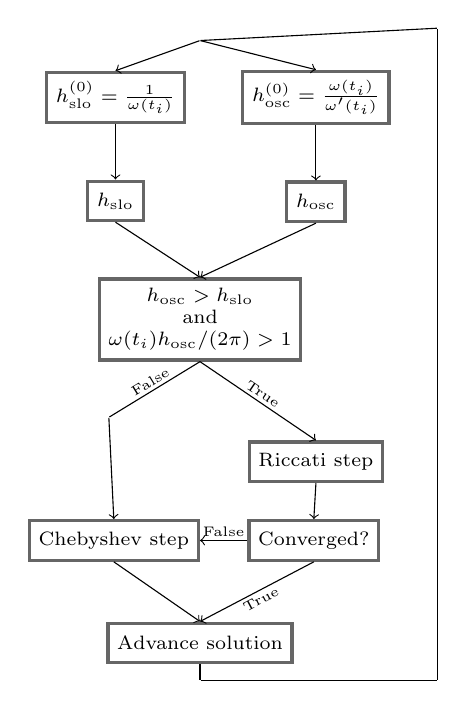
\begin{tikzpicture}[
    roundnode/.style={circle, draw=black!60, fill=green!0, very thick, minimum size=7mm},
    squarednode/.style={rectangle, draw=black!60, fill=red!0, very thick, minimum size=5mm},
    ]
    \tikzstyle{every node}=[font=\scriptsize]
    %Nodes
    \node[squarednode]      (hsloini)   {$h_{\text{slo}}^{(0)} = \frac{1}{\omega(t_i)}$};
    \node[squarednode]      (hoscini)  [right=0.7cm of hsloini] {$h_{\text{osc}}^{(0)} = \frac{\omega(t_i)}{\omega'(t_i)}$};
    \node[squarednode]      (hslo)  [below=0.7cm of hsloini] {$h_{\text{slo}}$};   
    \node[squarednode]      (hosc)  [below=0.7cm of hoscini] {$h_{\text{osc}}$};    
    \node[squarednode, align=center]      (switch) [below right=0.7cm and -0.6cm of hslo] {$h_{\text{osc}} > h_{\text{slo}}$ \\ and \\$\omega(t_i) h_{\text{osc}}/(2\pi) > 1$};
    \node[squarednode]      (ricc)  [below =4cm of hoscini] {Riccati step};  
    \node[squarednode]      (cheb)  [below left=2cm and -1.3cm of switch] {Chebyshev step}; 
    \node[squarednode]      (conv)  [right=0.6cm of cheb] {Converged?};     
    \node[squarednode]      (accept)  [below =3.3cm of switch] {Advance solution};    
    \node[inner sep=0, minimum size=0, below left=0.7cm and -0.15cm of switch] (k) {}; % invisible node
    \node[inner sep=0, minimum size=0, below=0.2cm  of accept] (l) {}; % invisible node
    \node[inner sep=0, minimum size=0, right=3cm of l] (m) {}; % invisible node
    \node[inner sep=0, minimum size=0, above=8.27cm of m] (n) {}; % invisible node
    \node[inner sep=0, minimum size=0, above=3cm of switch] (o) {}; % invisible node    
    
    %Lines
    \draw[->] (hsloini.south) -- (hslo.north);
    \draw[->] (hoscini.south) -- (hosc.north);
    \draw[->] (hosc.south) -- (switch.north);
    \draw[->] (hslo.south) -- (switch.north);
    \draw[->] (switch.south) -- (ricc.north) node[midway, above=-0.5ex, sloped] {\tiny True};    
    \draw[-] (switch.south) -- (k) node[midway, above=-0.5ex, sloped] {\tiny False};  
    \draw[->] (k) -- (cheb.north) ;
    \draw[->] (conv.south) -- (accept.north) node[midway, below=-0.5ex, sloped] {\tiny True};    
    \draw[->] (conv.west) -- (cheb.east) node[midway, above=-0.5ex] {\tiny False};
    \draw[->] (cheb.south) -- (accept.north);    
    \draw[->] (ricc.south) -- (conv.north);
    \draw[-] (accept.south) -- (l) ;
    \draw[-] (l) -- (m) ;    
    \draw[-] (m) -- (n) ;    
    \draw[-] (n) -- (o) ; 
    \draw[->] (o) -- (hsloini.north) ;
    \draw[->] (o) -- (hoscini.north) ;    
    
    \end{tikzpicture}  
    \end{minipage} 
\end{noframe}

\begin{noframe}
    Why it works: Residual\vfill
    \begin{minipage}{0.5\textwidth}
 	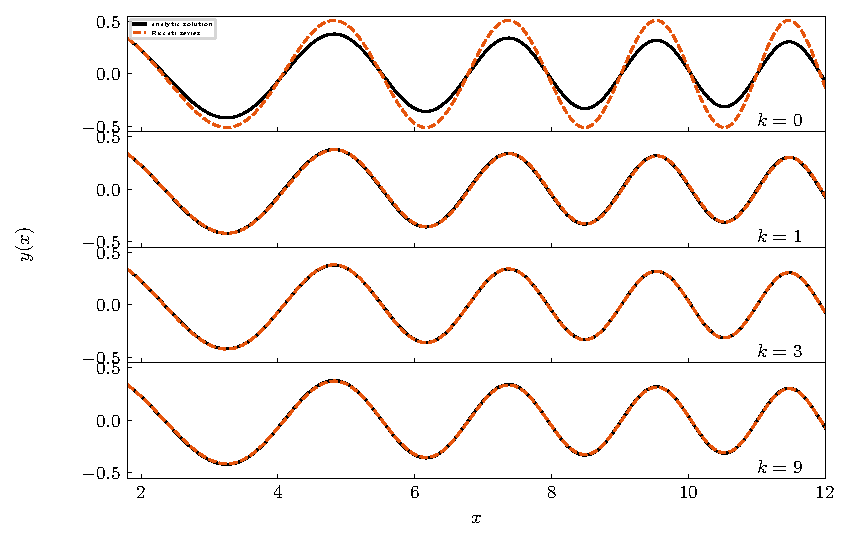
\includegraphics[]{residual.pdf}   
 	\end{minipage}\hfill
 	\begin{minipage}{0.5\textwidth}
 	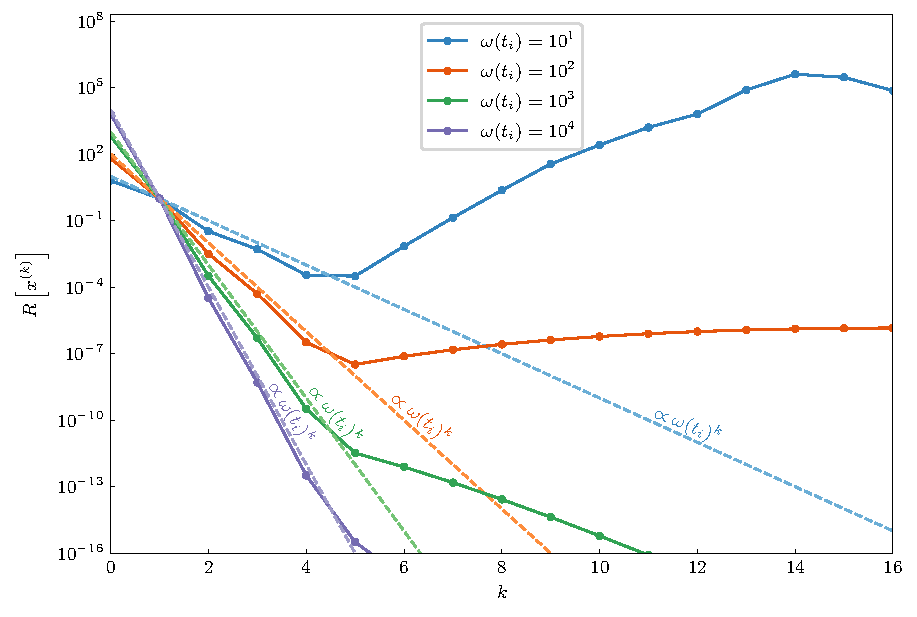
\includegraphics[]{residual-k.pdf}
 	\end{minipage}
\end{noframe}

\begin{noframe}
    Why it works II: a theorem \\
    \medskip
	\begin{theorem}[Temporary geometric convergence for small $\omega'/\omega$]
		\scriptsize For a given $t \in \mathbb{R}$ and $\omega$ analytic in the closed ball $B_\rho(t) := \{z\in\mathbb{C} : |z-t| \le \rho\}$ for some $\rho>0$, define the bounds 
  \begin{align}\label{eq:ommag}
  \eta_1 \le &|\omega(z)| \;\le\; \eta_2~, \quad \quad \quad \qquad \forall z\in B_\rho(t)~,
   \\
  &|\omega'(z)| \le \eta_3 \;\le\; \frac{\eta_1^2}{18}~,
  \qquad \forall z\in B_\rho(t)~.
  \label{eq:omder}
  \end{align}
  (i.e.\ $\omega'$ should be sufficiently small.)
  Let $k\in\{0,1,\dots\}$ be sufficiently small such that
  \begin{equation}
  r \equiv \frac{1}{2\tilde{\eta}_1 \rho}
  \biggl(1 + \frac{\tilde{\eta}_2}{\tilde{\eta}_1}\biggr) k + \frac{\eta_3}{4\tilde{\eta}_1^2}
  \; \le \; \frac{4}{5}
  \label{eq:r}
  \end{equation}
  where $\tilde{\eta}_1:=\eta_1 - 3\eta_3/\eta_1$ and $\tilde{\eta}_2:=\eta_2 + 3\eta_3/\eta_1$.
  Then after any number $j\le k$ of iterations of \eqref{eq:init}--\eqref{eq:iter},
  the function $x_j$ has Riccati residual \eqref{eq:R} bounded at the point $t$ by
  \begin{equation}
  |R_j(t)| \;\le\; \eta_3 r^j~.
  \end{equation}

	\end{theorem}
\end{noframe}


\begin{noframe}
    Why it works II: A theorem \\
    \medskip
    {\footnotesize
    \begin{itemize}
    \item{Theorem means that for sufficently small $\omega'/\omega$, can get geometric convergence up to $k$ iterations, }
    \item{But rate of convergence deteriorates with $k$ }
    \item{For there to exist any $k$ that satisfies conditions on $r$, $\omega$ has to have large lower bound $\rightarrow$ $t$ in oscillatory region of ODE}
    \end{itemize}
    }
    Proof \\
    {\footnotesize
    \begin{itemize}
    \item{Write down residual iteration: $R_{j+1}$ in terms of $R_{j}$}
    \item{Define the concentric nested set of closed balls $B_j = B_{\rho_j}(t)$, with radii $\rho_j = (1-j/k)\rho$, $j=0,1,\dots,k$ }
    \item{($B_0$ is original ball in theorem, $B_k$ is a single point)}
    \item{Bound $f'$ in $B_{j+1}$ in terms of $||f||_j = \max_{z \in B_j} |f(z)|$ by using Cauchy's theorem for derivatives, }
    \item{Prove by induction that for iteration $j$, 
    \begin{align}
    \tilde{\eta}_1 \leq &|x_l| \leq \tilde{\eta}_2 \quad \text{in} \; B_j, \quad \text{for all} \; l = 0, 1, \ldots, j, \\ 
    &|R_l| \leq \eta_3 r^{l} \quad \text{in} \; B_j, \quad \text{for all} \; l = 0, 1, \ldots, j.
    \end{align}
    }
    \item{Then apply these to the residual iteration.}
    \end{itemize}
    }

\end{noframe}

\begin{noframe}
    Future outlook \& conclusions \\
    \medskip
    {\footnotesize
    \begin{itemize}
    \item{An efficient method for solving general, linear, 2nd order ODEs, with a frequency that may be large,}
    \item{No other existing method that can deal with $\gamma \neq 0$ and nonoscillatory regime other than oscode }
    \item{oscode is anoher asymptotic solver, uses WKB expansion, but since WKB significantly more difficult to make adaptive (due to underlying recursion relation involving all previous terms, c.f.\ only 1 term here), only uses a fixed number of terms in the asymptotic expansion}
    \item{oscode is low-order, this method is arbitrarily high-order}
    \end{itemize}
   }
   {\footnotesize
    \begin{itemize}
    \item{Stepsize-update algorithm needs further refining}
    \item{Chebyshev spectral method could be further optimised via ultraspherical polynomials (cite Dan, chebops)}
    \item{Method has potential to generalise to PDEs}
    \end{itemize}
   }
\end{noframe}

%\begin{frame}[b]
%	But it doesn't understand where the logo is, which can look bad. One could adjust it so it does, but you sacrifice a lot of usable white space.
%\end{frame}

\end{document}
